\documentclass[12pt,a4paper]{article}

\usepackage{graphicx}
\usepackage{float}
\usepackage{amsmath}
\usepackage[noend]{algpseudocode}
\graphicspath{ {./images/} }
\renewcommand{\baselinestretch}{1.5}
\everymath{\displaystyle}

\author{Erik-Cristian Seulean}
\title{Nonparametric Bayesian inference - a guide to clustering algorithms}
\date{\today}

\begin{document}
\maketitle
\section{Motivation}

In the last years, in every corner of the internet there are enormous quantities of data created. 
Regardless of the nature of this data, as quantities increase over time, we're challenged to find
ways to group data into well-defined categories. The categorization of data allows us to explore 
datasets in a more organized way and reduces the time required to find particular datapoints. 
Today, there are over 6 million articles on Wikipedia. Regardless of the size of this article
collection, everything is grouped in ways that allows us to explore different interests in
organized ways. The library, here in St. Andrews contains over 1 million books, yet finding a book
today on a topic such as Bayesian inference is a matter of minutes. As the University increases the
diversity of degrees that students can take, the number of book categories increase over time and 
this leads to the following question \textit{How do we generate a mathematical model that is capable
to group books that are alike into well-defined categories ?}

\section{Nonparametric Bayes a brief description}
There are two separate classes of Bayesian inference. One class contains inference on
parameters of distributions, where the prior and posterior distributions are functions of parameters of
interest with fixed dimension. In this case we can consider the following: 

\begin{itemize}
    \item $\theta = (\theta_{1}, \theta_{2}, ..., \theta_{n})$ - the parameter that we are interested in 
    \item $P(\theta)$ - prior probability
    \item $\pi(\theta|X)$ - posterior probability
\end{itemize}

In the above example, the parameter has a fixed determined dimension. We know what probability distributions
work for the number of parameters we have. For a single unknown parameter for example we can use a Uniform, 
Poission or Exponential distribution. For two parameters we could use a Normal or Beta distribution (among others)
depending on what sort of data we are modelling. 
In this situation we can use Bayes formula to define the posterior distribution based on the prior and likelihood:

$$\pi(\theta|x_{1}, x_{2}, ..., x_{n}) \propto \prod_{i}^{n}f(x_{i}|\theta)p(\theta)$$ 

But what happens when you don't know beforehand how many parameters you need ? How many parameters will describe
your data well ? Are your observations dependent on one parameter or 3 parameters ? Nonparametric Bayesian analysis
is focused on problems where the number of parameters are not known beforehand. In other words, we can assume that
there can be any number of parameters, we will examine the data and draw some conclusions on how many parameters of 
interest describe the data well. 
In more rigorous mathematical terms, so far we can define the following:

\begin{itemize}
    \item $X_{1}, X_{2}, X_{3}, ... X_{n}$ are i.i.d observations from an \textit{unknown} distribution F
    \item F is not from a finite space, we cannot index it with a finite number of parameters
\end{itemize}

Similar to the parametric case, we would like to apply Bayesian methods. This means that we need to 
specify a prior distribution, but because we don't know the number of parameters that we are dealing with,
we cannot specify priors on parameters, we need to specify a prior on the distribution itself. What in 
the parametric case was $P(\theta)$ becomes now $P(F)$ where F is a distribution! 
To put it in the context of the example from the beginning of the essay, if we start making an analysis on
the topics of the books in the library, the more books we examine the more topics we can encounter. That doesn't
mean that every book is a new topic, but the number of topics grows as we examine more books. This is equivalent
to the number of parameters in a nonparametric Bayesian model where the number of parameters is unknown but growing
with the data. 

\section{The clustering problem}
Assuming we have observations $X_{1}, X_{2}, ..., X_{n}$ we want to assign every datapoint to a single cluster.

\begin{figure} [H]
    \begin{center}
        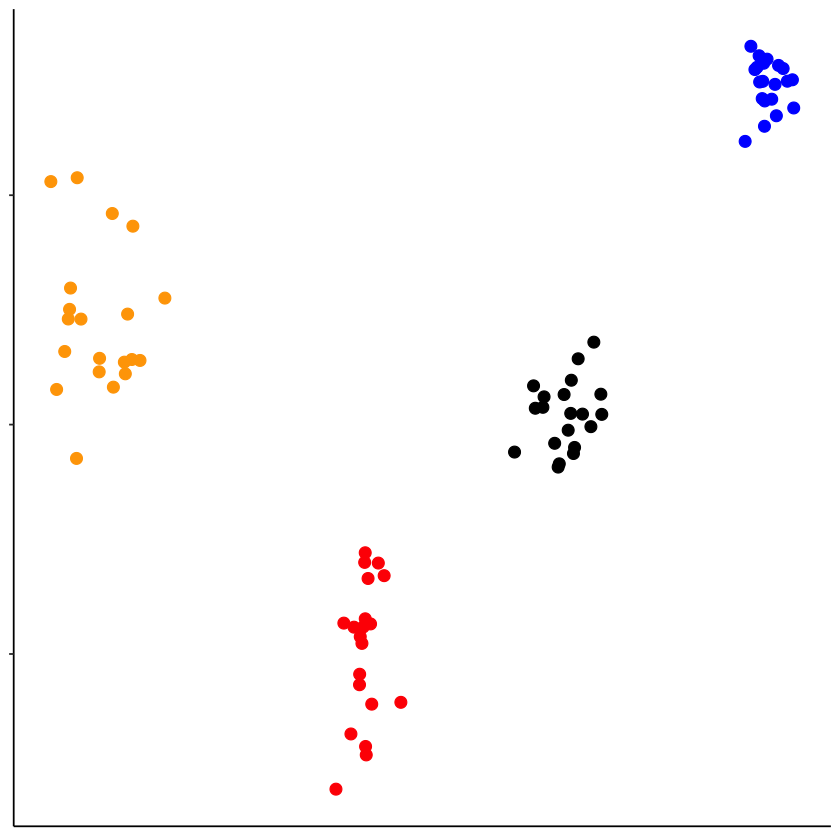
\includegraphics[scale=0.3, width=5cm]{clusters.png}
        \caption{Clustered datapoints}
        \label{fig:boat1}
    \end{center}
\end{figure}

In a general Gaussian mixture model, with the number of clusters $K$ set to 2, we could potentially have the following setup: 

$$\mu_{k} \sim \mathcal{N}(\mu_{0}, \sigma_{0}^2)$$ 
$$\rho_{1} \sim Beta(a, b)$$
$$\rho_{2} = 1 - \rho{1}$$ 
$$Z_{n} \sim Categorical(\rho_{1}, \rho_{2})$$
Here we're choosing $\rho_{1}$ coming from a Beta distribution as it is mathematically convenient, but in practice, it would require further analysis to figure out if this is a valid assumption. Depending on the parameters of this Beta distribution, it would put more or less mass on $\rho_{1}$ compared to $\rho_{2}$.

In case we want to generalize the model above to have K clusters, we can replace the Beta distribution above with a Dirichlet distribution. In this case, instead of drawing only one observation for $\rho_{1}$, we could draw K observation for $\rho_{1}, \rho_{2}, \rho_{3}, ..., \rho_{K}$.

$$\mu_{k} \sim \mathcal{N}(\mu_{0}, \sigma_{0}^2)$$ 
$$\rho_{1:K} \sim Dirichlet(a_{1}, a_{2}, ..., a_{K})$$
$$Z_{n} \sim Categorical(\rho_{1}, \rho_{2}, ... ,\rho_{K})$$

The Dirichlet distribution used above is the natural generalization of Beta distribution to a multiparameter case:

$$ Dir(\rho_{1}, \rho_{2}, ..., \rho_{n}| a_{1}, a_{2}, ..., a_{n}) = \frac{\Gamma(\sum_{i=1}^{K}a_{i})}{\prod_{i=1}^{K}\Gamma(a_{i})}\prod_{i}^{K}\rho_{i}^{a_{i} - 1}$$ where
$\sum_{i}^{K} \rho_{i} = 1, a_{k} > 0$ and $\rho_{k} \in (0, 1)$.

The \textit{rdirichlet} function provided with the library can generate samples from a Dirichlet distribution.

So far the examples above, all work on the case where the number of clusters is fixed and known. We are capable of drawing observations from the Dirichlet distribution, because we know how many parameters we are working with. In the figure below, the first delimitation corresponds to the first cluster, second to the second cluster and so on, up to 100 clusters.

\begin{figure} [H]
    \begin{center}
        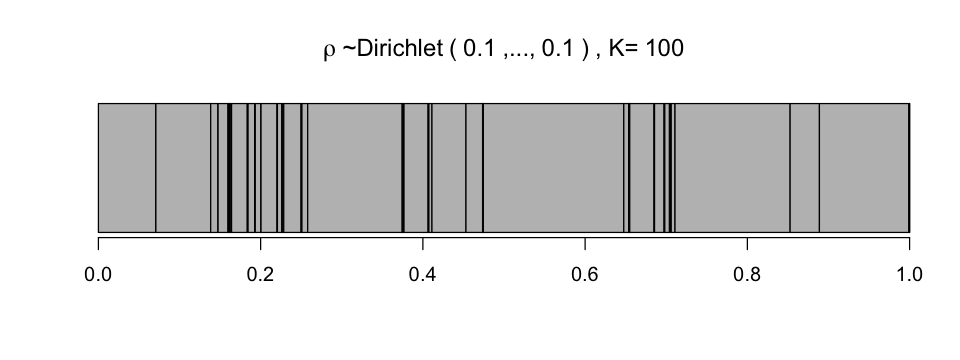
\includegraphics[scale=1, width=5cm]{stacked_dirichlet.png}
        \caption{Clusters generated from a Dirichlet distribution.}
        \label{fig:stacked_dirichlet}
    \end{center}
\end{figure}

At this point, we only considered the available clusters, but we have not sampled our datapoints $X_{1}, X_{2}, ..., X_{n}$ into the corresponding clusters. To put a particular datapoint into a certain cluster, we can draw an observation from a Uniform distribution and check which cluster it belongs to. We can repeat the same until all n datapoints are assigned to a cluster. The cluster generation function in the library allows to visually get an intuition of how this happens sequentially. 

\begin{figure} [H]
    \begin{center}
        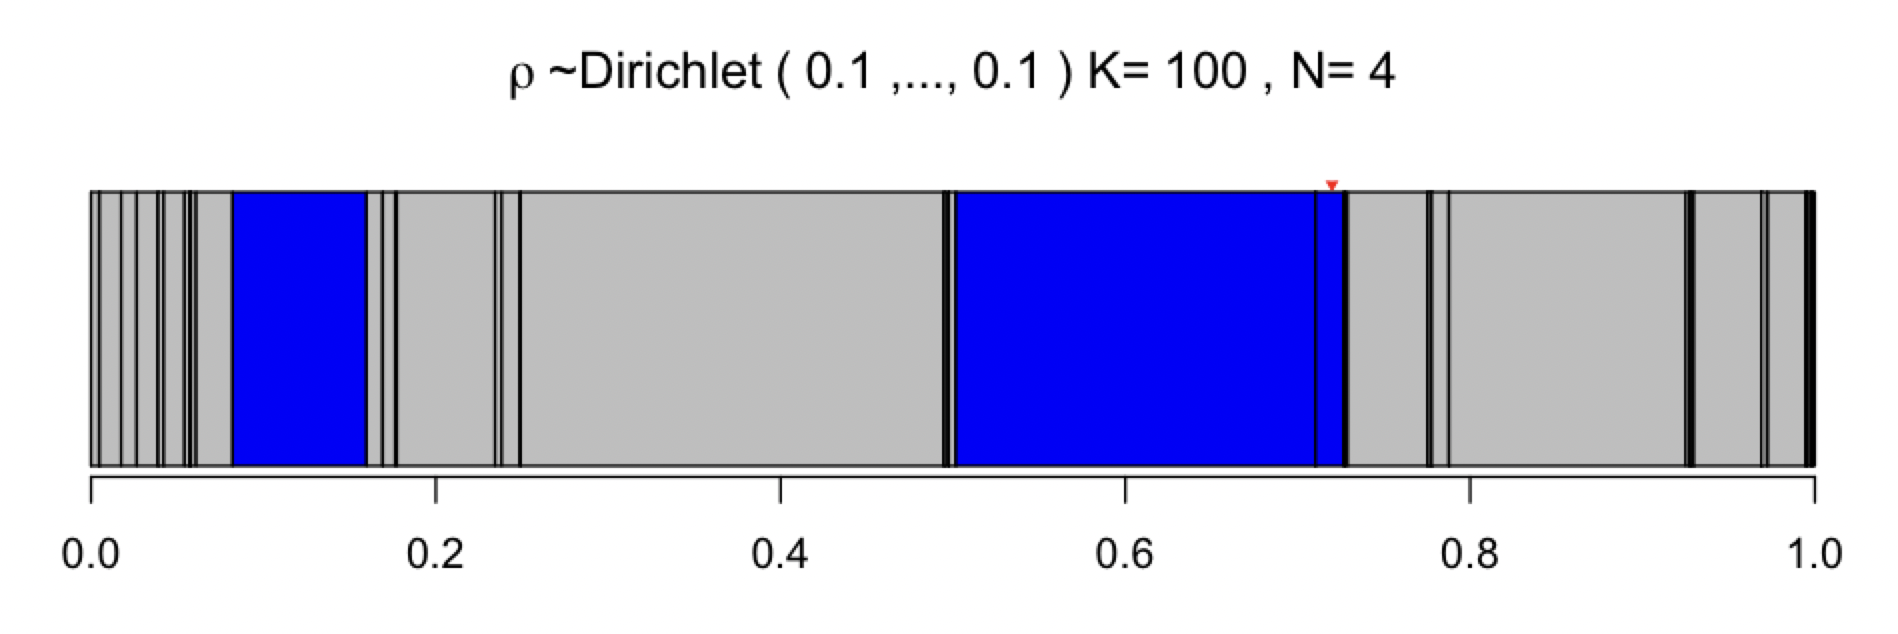
\includegraphics[scale=1, width=5cm]{clustered_points.png}
        \caption{Clustered points}
        \label{fig:clustered_points}
    \end{center}
\end{figure}

While this model looks appealing, there is always going to be an upper bound on K, that defines the number of clusters. In this scenario, there is no reliable way to choose K that would be sufficient in any general case. Even if we can come up with a value of K large enough, there are computational concerns when it comes to storing a large amount of information in memory that is associated with K.

\section{Setting K=$\infty$}
A solution to the above limitation is to set K to be arbitrary large that would not limit us from having a very large number of clusters. In this case we need a different procedure to generate $\rho_{1}, \rho_{2}, ..., \rho_{K}$ from a Dirichlet distribution. What we want to do is take the interval $(0, 1)$ and break it into an infinite number of subintervals that sum up to 1. In other words, we first break a proportion of the interval $(0, 1)$ and denote that being $\rho_{1}$. Out of the remaining part $(\rho_{1}, 1)$ we break another proportion and denote that to be $\rho_{2}$. We can repeat this as many times as we want, and we can generate an infinite number of proportions, that sum up to 1, the length of the initial interval. This algorithm is called the \textit{"stick-breaking process"} and can be summarized as follows: 

\begin{itemize}
    \item Generate $P_{1} \sim Beta(a_{1}, b_{1})$. Set $\rho_{1}$ to this value.  
    \item Generate $P_{2} \sim Beta(a_{2}, b_{2})$. Set $\rho_{2} = (1 - P_{1})P_{2}$
    \item Generate $P_{3} \sim Beta(a_{3}, b_{3})$. Set $\rho_{3} = (1 - P_{1})(1-P_{2})P_{3}$
    \item Set $\rho_{K} = 1 - (\rho_{1} + \rho_{2} + ... + \rho_{K-1})$
\end{itemize}

The choice of parameters $a$ and $b$ for the Beta distribution are researched by Ishwaran and James, 2001, and we will simply use $1$ and $\alpha$ with $\alpha$ given for all $a_{k}$ and $b_{k}$. 
When $a_{k}=1$ and $b_{k}=\alpha$, $\alpha > 0$ the process is called \textit{Dirichlet process stick-breaking}. The distribution over all $\rho = (\rho_{1}, \rho_{2}, ...)$ is called Griffin-Engen-McCloskey (GEM). 

$$ (\rho_{1}, \rho_{2}, ...) \sim GEM(\alpha)$$

\section{Dirichlet process mixture model}

The Gaussian mixture model specified above, for K fixed clusters can be transformed to work with an arbitrary number of clusters by using the $GEM$ distribution instead of Dirichlet.

$$(\rho_{1}, \rho_{2}, ...) \sim GEM(\alpha)$$
$$\mu_{k} \sim \mathcal{N}(\mu_{0}, \sigma^2)$$
$$ G = \sum_{k}^{\infty}\rho_{k}\delta_{\mu k} \sim DPM(\alpha, \mathcal{N}(\mu_{0}, \sigma^2))$$

The above will put weight $\rho_{k}$ at $\delta_{\mu k}$ where $\delta_{\mu k}$ denotes the $k^{th}$ cluster. The first parameter is $\alpha$, parameter needed for the GEM distribution, the second one is the distribution used to draw $\delta_{\mu k}$, the locations of the clusters. In practice, sampling from this distribution would mean that with probability $\rho_{k}$ will draw an observation from cluster with center $\delta_{\mu k}$.

The problem that arises with this model is that we cannot draw an infinite number of probabilities $\rho_{k}$, but we can do draw them on demand, as we sample. The example above, where we draw points into the cluster, by sampling from a Uniform distribution and check which clusters the points belong to can give an indication of what we can do here. If we first draw a point $u \sim Uniform(0, 1)$ we can then sample enough $\rho_{k}$ values that would make the sum of all $\rho_{k}$ sampled be greater than $u$. The complete step by step sampling algorithm is given by the following:

\begin{enumerate}
    \item Draw an observation $u$ from a $Uniform(0, 1)$ distribution.  
    \item Generate $P_{k} \sim Beta(1, \alpha)$ and find $\rho_{k}$ using the \textit{stick breaking algorithm}. Repeat until $\sum_{k}\rho_{k} > u$. 
    \item For every $\rho_{k}$ sampled, sample the center for the cluster associated with $\rho_{k}$ from $\mathcal{N}(\mu_{0}, \sigma_{0}^2)$ 
    \item Find the cluster the point belongs to such that $\rho_{k-1} < u < \rho_{k}$.
    \item Sample an observation from $\mathcal{N}(\mu_{k}, \sigma^2)$ where $\mu_{k}$ is the center of the cluster that was selected.
    \item Repeat until all $n$ points are sampled.
\end{enumerate}

The algorithm above can be observed step by step using \textit{rDPMM\_visual} in the package provided, while \textit{rDPMM} returns a sample.

The \textit{Dirichlet process} as presented above, is a distribution of distributions over a sample space. If we consider $A_{1}, A_{2}, ..., A_{n}$ a partition of the sample space $\Omega$, we can say that the $Dirichlet\ process$ assigns a particular mass, to each of this partitions of the sample space. The total mass distributed to each partition is distributed following a \textit{Dirichlet\ distribution}. 

$$(P(A_{1}), P(A_{2}), ... , P(A_{k})) \sim Dir(\alpha G(A_{1}), \alpha G(A_{2}), ..., \alpha G(A_{k}))$$
Given that there is a connection between the \textit{Dirichlet process} and the \textit{Dirichlet distribution}, we can derive the posterior distribution when we have Dirichlet-Categorical or Dirichlet-Multinomial prior and likelihood pairs:

$$\rho_{1}, ... ,\rho_{k} \sim Dir(\alpha_{1}, ..., \alpha_{k})$$
$$x_{1}, ... ,x_{k} \sim Categorical(\rho_{1}, ... \rho_{k})$$

$$\displaystyle \pi(\rho|x) \propto f(x|\rho)\pi(\rho) \propto \prod_{i}^{k} f(x_{i}| \rho)\pi(\rho) $$
$$\propto \prod_{i}^k \prod_{j}^k \rho_{j}^{I(x_{i} = j)}\prod_{i}^k \rho_{i}^{\alpha_{i} - 1} \propto \prod_{j}^k \rho_{j}^{\sum_{i}I(x_{i} = j)}\prod_{i}^k \rho_{j}^{\alpha_{j} - 1}$$
$$ \propto \prod_{j}^k \rho_j^{{c_{j}} + \alpha{j} - 1}$$
$c_{j} = \sum_i I(x_{i} == j) $

Similarly, if the observations are from a \textit{Multinomial distribution}:
$$x_{1}, ... ,x_{k} \sim Multinomial(\rho_{1}, ... \rho_{k})$$
$$\displaystyle \pi(\rho|x) \propto f(x|\rho)\pi(\rho) \propto \prod_{i}^{k} f(x_{i}| \rho)\pi(\rho) $$
$$ \propto \prod_{i}^{k} \rho_{i}^{c_{i}} \prod_{i}^{k} \rho_{i}^{\alpha - 1} \propto \prod_{i}^{k} \rho_{i}^{c_{i} + \alpha_{i} - 1}$$ 

In both cases, we can notice that the posterior is following a \textit{Dirichlet distribution} so the Dirichlet distribution is the Conjugate prior for both the Categorical and the Multinomial distributions. The posterior distribution in these cases is $\pi(\rho|x) \sim Dir(\alpha_{1} + c_{1}, ..., \alpha_{k} + c_{k})$. In terms of the clusters (or partition of the sample space), if we observe a new observation in cluster $i$, the posterior then is updated with a new observation in cluster $i$:
$$(P(A_{1}), P(A_{2}), ... , P(A_{k})) \sim Dir(\alpha G(A_{1}), \alpha G(A_{2}), ..., G(A_{i}) + 1, ..., \alpha G(A_{k}))$$ which in fact leads to $ G|x_{1} \sim DP(\alpha + 1, \frac{\alpha \mathcal{N} + \delta_{x}}{\alpha + 1})$.

\section{Pólya Urn}

In the section above, drawing observations from the \textit{Dirichlet process} required to sample values for $\rho_{k}$ from the \textit{GEM distribution}. If we could find a way to avoid this step, we could remove the $\rho_{k}$ variables altogether and the model would be simpler. It turns out that there is a way of doing this by integrating out $\rho_{k}$. As before, we could start from the same setup as in the Gaussian mixture model:

$$\rho_{1} \sim Beta(a, b)$$
$$Z_{n} \sim Categorical(\rho_{1}, \rho_{2})$$

\begin{align*}
\begin{array}{l@{{}={}}l}
    P(Z_{n} = 1|Z_{1}, Z_{2}, ..., Z_{n-1})
    & \int P(Z_{n} = 1, \rho_{1}|Z_{1}, Z_{2}, ..., Z_{n-1}) \,d\rho_{1} \\
    & \int P(Z_{n} = 1|\rho_{1})P(\rho_{1}|Z_{1}, Z_{2}, ..., Z_{n-1}) d\rho_{1} \\
    & \int \rho_{1} Beta(a + c_{1}, b + c_{2})d\rho_{1} \\
    & \int \rho_{1} \frac{\Gamma(a + c_{1} + b + c_{2})}{\Gamma(a+c_{1})\Gamma(b+c_{2})}\rho_{1}^{a+c_{1}}(1-\rho_{1})^{b+c_{2}} d\rho_{1} \\
    & \frac{\Gamma(a + c_{1} + b + c_{2})}{\Gamma(a+c_{1})\Gamma(b+c_{2})} \frac{\Gamma(a+c_{1}+1)\Gamma(b+c_{2})}{\Gamma(a + c_{1} + b + c_{2}+1)} \\
    & \frac{a + c_{1}}{a + c_{1} + b + c_{2}}
\end{array}
\end{align*}

where $c_{j} = \sum_{i}^{n-1}I(Z_{i} = j)$

In this case we are independent on $\rho_{k}$, and we can put an observation $Z_{k}$ into the cluster one with probability derived above. Intuitively, this can be interpreted in the following way. If we start with an urn, containing initially \textit{a} number of red balls and \textit{b} blue balls and draw from a \textit{Bernoulli distribution} with probability derived above, we can keep adding red or blue balls to the urn, based on the value sampled. As the number of balls in the urn goes to infinity, the proportion of red balls in the urn is $\rho_{1}$. An alternative intuition is that using the initial setup, we can draw a ball from the urn inspect the color and return to the urn two balls of that same color. As the number of balls grows to infinity the proportion of red balls goes to $\rho_{1}$. Not just the proportion of red to blue balls is $\rho_{1}$ as the number of balls goes to infinity, the distribution of the proportion of red balls is also \textit{Beta(a, b)}. The distribution of red balls in the urn is noted as being \textit{PólyaUrn(a, b)}.

The Pólya urn for two types of balls can be generalized to K different colors, but instead of using Beta we can use $\rho_{1}, ..., \rho_{k} \sim Dirichlet(\alpha_{1}, ..., \alpha_{k})$. The probability of $n^{th}$ observation to go into cluster k given the previous \textit{n-1} observations is the same:
$P(Z_{n} = k|Z_{1}, ..., Z_{n-1}) = \frac{\alpha_{k} + c_{k}}{\sum_i^n (\alpha_{i} + c_{i})}$ . If we keep adding balls to the urn, in the same procedure as above, the proportion of balls in the urn will follow the \textit{Dirichlet distribution} that we started with. 

As before, we built the model up starting with a \textit{Beta distribution} for two clusters, then we generalized to K clusters using a \textit{Dirichlet distribution}. The next logical step is to set $K=\infty$. To be able to handle an arbitrary number of clusters, we will use a different type of urn called \textit{Hoppe urn} or \textit{Blackwell-MacQueen urn}. The urn will initially contain only one magic ball. When the magic ball is extracted from the urn, we put it back together with a ball of a new color, that does not exist in the urn. If we extract a ball of a particular color, we will return it to the urn together with another ball of the same color. The distribution of balls of any color is \textit{PólyaUrn(1, $\alpha$)}. The proportion of balls of the first color is also $Beta(1, \alpha)$, and this takes us back to the \textit{Stick breaking process.} If we consider $\rho_{k}$ the proportion of balls of the $k^{th}$ color we have the following: 

$$ V_{k} \sim Beta(1, \alpha) $$
$$\rho_{1} = V_{1}$$
$$\rho_{2} = (1 - V_{1})V_{2}$$
$$\rho_{k} = \prod_{i=1}^{k-1}(1-V_{i})V_{k}$$

The urn is identical to the Dirichlet process, but we don't have to deal with the \textit{GEM distribution} anymore as the $\rho_{k}$ were integrated out.

\section{The chinese restaurant process}
The \textit{chinese restaurant process} works in the same way as the \textit{Pólya urn}. A customer walks into a restaurant and either sits down at a new table or sits at a table that is already occupied, proportional to the number of people that already sit at the table. This process is identical to the Pólya urn, we can either draw the magic ball (sit at a new table) or draw a different colored ball (sit at an already occupied table). Each table in this case will have a color, and as in the previous example we have infinitely many tables. A librarian working at the library in St. Andrews, can either assign a new book to an existing category or create a new category for that book. 

It comes naturally to ask what is the difference between the \textit{Dirichlet process} and the \textit{Chinese Restaurant process}. While the \textit{Dirichlet process} describes both the cluster assignments and the proportion of the clusters the \textit{Chinese Restaurant process} describes only the cluster assignments. In many applications, knowing the cluster proportions is not of much use, so applications generally rely on implementations of the CRP algorithm for practical purposes. I was curious to find out where the name for the algorithm comes from, and I found out that the Chinese restaurants in San Francisco, in the nineties were trying to accommodate as many customers as possible. Customers were generally interested in the popular tables (with many other customers) but now and then, a customer would come in and sit at a new table. 

Given that we are only considering the cluster arrangements and not the proportions for each cluster, we are interested in modelling the partitions of the datapoints. For example, one partition of 10 datapoints can be the following $\{\{1, 5, 7\}, \{2,3,4,6\}, \{8, 9\}\}$. That denotes that the first datapoint, the $5^{th}$ and the $7^{th}$ are assigned in cluster one, and so forth. The order of the clusters doesn't matter, as the clusters are interchangeable, the datapoints will be associated with the same cluster regardless. It comes naturally to ask what is the probability of a cluster arrangement. The probability for the cluster arangement above is the following: $$\frac{\alpha}{\alpha}\frac{\alpha}{\alpha+1}\frac{1}{\alpha+2}\frac{2}{\alpha+3}\frac{1}{\alpha+5}\frac{3}{\alpha+6}\frac{2}{\alpha+7}\frac{\alpha}{\alpha+8}\frac{1}{\alpha+9}$$

From here we can easily generalise to N datapoints. Considering K clusters and $n_{k}$ datapoints in cluster k we have the following: $$\frac{\alpha^{K} \prod_{k}(n_{k}-1)!}{\alpha(\alpha+1)...(\alpha+N-1)} = P(\prod\nolimits_{N} = \pi_{N})$$

We notice here that the order in which datapoints are assigned to clusters doesn't change the probability of a particular arrangement. If we observe the partition of the 10 datapoints as above, the probability for the partition is the same if we permute the datapoints and consider them in a different order, as long as the datapoints are assigned to the same clusters as initially. This gives a property called exchangeability that comes handly in Gibbs sampling, which will be discussed in the later pages. This allows us to consider any datapoint, as being always the last one: 
$$P(\prod\nolimits_{N}|\prod\nolimits_{N, -n})= \left \{
    \begin{array}{ll}
		\frac{\#C}{\alpha+ N - 2} & \mbox{if joins cluster k} \\
		\frac{\alpha}{\alpha+N-2} & \mbox{if starts a new cluster} 
	\end{array}
\right. $$ Where $\#C$ denotes the number of datapoints in that cluster until this point.

\section{Gibbs sampling for the Chinese restaurant process}

\end{document}\models